\section{Dassault/Dornier Alpha Jet}

\noindent
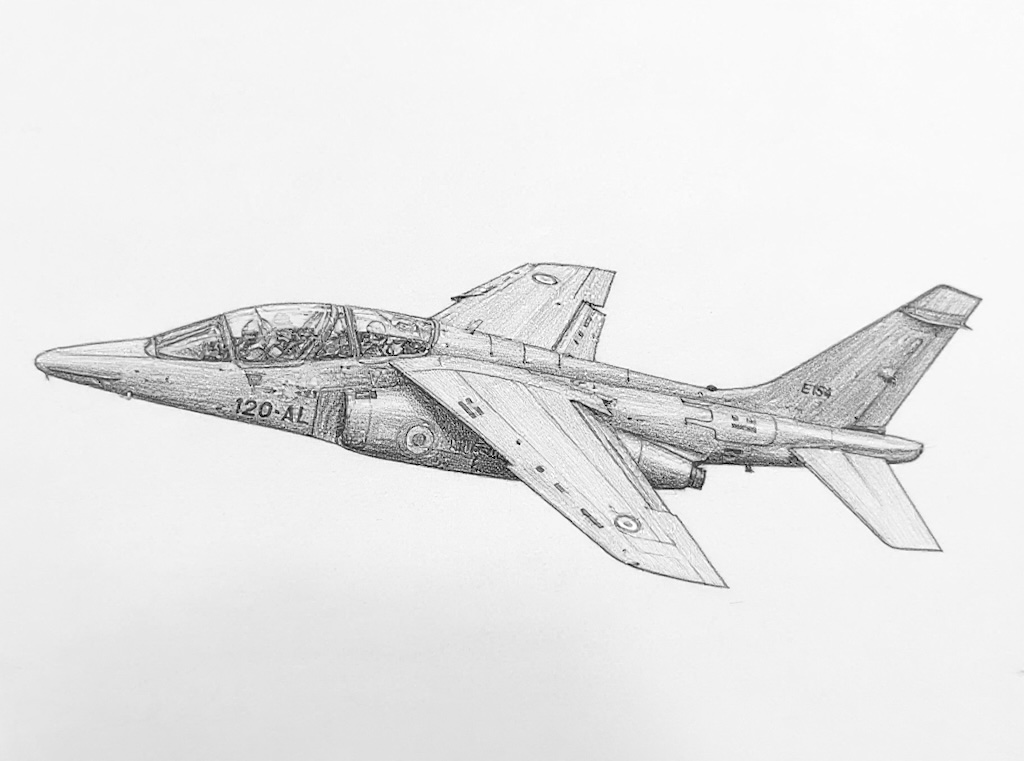
\includegraphics[width=\linewidth]{Alpha Jet.jpg}

\noindent
The Dassault/Dornier Alpha Jet is a two-seat advanced trainer and light attack aircraft. It was developed starting in 1967 and entered service in 1979.%
\note{Sources}{
    \begin{itemize}
        \item Goebel, \href{https://airvectors.net/avalpha.html}{Air Vectors}
        \item \href{https://en.wikipedia.org/wiki/Dassault Dornier_Alpha_Jet}{Wikipedia on the Alpha Jet}
        \item \href{https://en.wikipedia.org/wiki/DEFA_cannon}{Wikipedia on the DEFA cannon}
        \item \href{https://en.wikipedia.org/wiki/Gun_pod\#Examples}{Wikipedia on Gun Pods}
    \end{itemize}

    \noteparagraph{Photo Credit}
    \begin{itemize}
        \item\href{https://commons.wikimedia.org/wiki/File:Alpha_Jet_-_RIAT_2009_(croppped).jpg}{Tim Felce} (CC CC BY 2.5)
    \end{itemize}
}

\subsection{Versions}

\subsubsection{Alpha Jet E}

The Alpha Jet E is the trainer version, with the E designation taken from \emph{École} (school). It is equipped with two underwing and one centerline weapon stations, but in French and Belgian service these were intended only for weapons training. Some of its later users employed it as a light strike aircraft, despite its shortcomings compared to aircraft dedicated to this role.%
\note{Alpha Jet E ADC}{
    {\AirStr} has an ADC for the E (as a variant of the A). The ADC here is based on Chris Perleberg's update incorporating the changes in APJ 21.
}

It initially served in the French Armée de l’air and the Belgian Air Force, but later with the air forces of Egypt, Morocco, Nigeria, Qatar, Togo, Côte d’Ivoire, and with private companies.%
\note{Alpha Jet E Service and Combat}{
    Wikipedia.
}

\subsubsection{Alpha Jet A}

The Alpha Jet A is the attack version, with the A designation taken from \emph{Appui Tactique} (tactical support). Although very similar to the E, the A has two additional underwing weapon stations, a more advanced weapon system, and can replace the rear crew member with an ECM suite.%
\note{Alpha Jet A ADC}{
    {\AirStr} has an ADC for the E. The ADC here is based on Chris Perleberg's update incorporating the changes in APJ 21.
}

It initially served in the German Luftwaffe, replacing the Fiat G91R/3. After the end of the Cold War many of these aircraft were sold to the air forces of Portugal and Thailand.%
\note{Alpha Jet A Service}{
    Wikipedia.
}

\subsection{Armament and Stores}

The Alpha Jet has no internal guns, but when armed would typically carry a gun pod on the centerline station, normally a
CC420 30 mm DEFA pod for E models or a 27 mm Mauser pod for A models. The gun pod was originally not jettisonable, but this restriction was lifted by the 1989 upgrade of Luftwaffe Alpha Jet As.%
\note{Gun Pods}{
    \begin{itemize}
        \item For the A: Single Mauser 27 mm GP (Goebel) with 150 rounds (Wikipedia). The rate of fire is 1000-1700 RPM, which corresponds to 4.5 to 2.6 ammo points. An upgrade in 1989 which Luftwaffe As the ability to jettison the gun pod (Wikipedia).
        \item For the E: Single DEFA 30 mm GP (Goebel) with 150 rounds (Wikipedia). The model is the DEFA 553 (Wikipedia on DEFA). The rate of fire is 1300 RPM, which corresponds to 3.5 ammo. It may have been a CC420 gun pod (Wikipedia on gun pods).
    \end{itemize}
}

Typical stores would be SNEB 68~mm or CRV7 70~mm RPs or HE or cluster bombs.%
\note{Stores}{

    Stores include Matra \binarymultiply{18}{68 mm} or CRV7 \binarymultiply{19}{70 mm} RPs, AIM-9s, Matra Magics, and Mavericks, bombs including the BL755 cluster bomb (Wikipedia). However, the Maverick capability seems to not have been implemented.

    Could carry FTs with capacities of 310L (82 US gal) or 450L (119 US gal) (Goebel).

    The ICE upgrade to the A was to provide compatibility with Mavericks, but this was cancelled in 1988 and a more austere upgrade from 1989 gave the AIM-9Ls and the ability to jettison the gun pod (Wikipedia).

    Goebel states: “The French qualified a film-camera pod”.

}

\subsection{Combat}

The Alpha Jet A does not seem to have seen combat, but the Alpha Jet E has in Moroccan and Nigerian service, in the former case against Polisario Front in the Western Sahara War and in the latter against the Boko Haram militant group.

\subsection{ADCs}

\begin{adclist}
    \adcitem{Alpha Jet A}
    \adcitem{Alpha Jet E}
\end{adclist}

\clearpage
\listofnotes
